% --------------------------------------------------------------------------- %
% Poster for the ECCS 2011 Conference about Elementary Dynamic Networks.      %
% --------------------------------------------------------------------------- %
% Created with Brian Amberg's LaTeX Poster Template. Please refer for the     %
% attached README.md file for the details how to compile with `pdflatex`.     %
% --------------------------------------------------------------------------- %
% $LastChangedDate:: 2011-09-11 10:57:12 +0200 (V, 11 szept. 2011)          $ %
% $LastChangedRevision:: 128                                                $ %
% $LastChangedBy:: rlegendi                                                 $ %
% $Id:: poster.tex 128 2011-09-11 08:57:12Z rlegendi                        $ %
% --------------------------------------------------------------------------- %
\documentclass[a0paper,portrait]{baposter}

\usepackage{relsize}		% For \smaller
\usepackage{url}			% For \url
\usepackage{epstopdf}	% Included EPS files automatically converted to PDF to include with pdflatex

%%% Global Settings %%%%%%%%%%%%%%%%%%%%%%%%%%%%%%%%%%%%%%%%%%%%%%%%%%%%%%%%%%%

\graphicspath{{pix/}}	% Root directory of the pictures 
\tracingstats=2			% Enabled LaTeX logging with conditionals

%%% Color Definitions %%%%%%%%%%%%%%%%%%%%%%%%%%%%%%%%%%%%%%%%%%%%%%%%%%%%%%%%%

\definecolor{bordercol}{RGB}{40,40,40}
\definecolor{headercol1}{RGB}{186,215,230}
\definecolor{headercol2}{RGB}{80,80,80}
\definecolor{headerfontcol}{RGB}{0,0,0}
\definecolor{boxcolor}{RGB}{186,215,230}

%%%%%%%%%%%%%%%%%%%%%%%%%%%%%%%%%%%%%%%%%%%%%%%%%%%%%%%%%%%%%%%%%%%%%%%%%%%%%%%%
%%% Utility functions %%%%%%%%%%%%%%%%%%%%%%%%%%%%%%%%%%%%%%%%%%%%%%%%%%%%%%%%%%

%%% Save space in lists. Use this after the opening of the list %%%%%%%%%%%%%%%%
\newcommand{\compresslist}{
	\setlength{\itemsep}{1pt}
	\setlength{\parskip}{0pt}
	\setlength{\parsep}{0pt}
}

%%%%%%%%%%%%%%%%%%%%%%%%%%%%%%%%%%%%%%%%%%%%%%%%%%%%%%%%%%%%%%%%%%%%%%%%%%%%%%%
%%% Document Start %%%%%%%%%%%%%%%%%%%%%%%%%%%%%%%%%%%%%%%%%%%%%%%%%%%%%%%%%%%%
%%%%%%%%%%%%%%%%%%%%%%%%%%%%%%%%%%%%%%%%%%%%%%%%%%%%%%%%%%%%%%%%%%%%%%%%%%%%%%%

\begin{document}
\typeout{Poster rendering started}

%%% Setting Background Image %%%%%%%%%%%%%%%%%%%%%%%%%%%%%%%%%%%%%%%%%%%%%%%%%%
\background{
	\begin{tikzpicture}[remember picture,overlay]%
	\draw (current page.north west)+(-2em,2em) node[anchor=north west]
	{
\includegraphics[height=1.1\textheight]{background}};
	\end{tikzpicture}
}

%%% General Poster Settings %%%%%%%%%%%%%%%%%%%%%%%%%%%%%%%%%%%%%%%%%%%%%%%%%%%
%%%%%% Eye Catcher, Title, Authors and University Images %%%%%%%%%%%%%%%%%%%%%%
\begin{poster}{
	grid=false,
	% Option is left on true though the eyecatcher is not used. The reason is
	% that we have a bit nicer looking title and author formatting in the headercol
	% this way
	eyecatcher=false, 
	borderColor=bordercol,
	headerColorOne=headercol1,
	headerColorTwo=headercol2,
	headerFontColor=headerfontcol,
	% Only simple background color used, no shading, so boxColorTwo isn't necessary
	boxColorOne=boxcolor,
	headershape=roundedright,
	headerfont=\Large\sf\bf,
	textborder=rectangle,
	background=user,
	headerborder=open,
  boxshade=plain
}
%%% Eye Cacther %%%%%%%%%%%%%%%%%%%%%%%%%%%%%%%%%%%%%%%%%%%%%%%%%%%%%%%%%%%%%%%
{
	Eye Catcher, empty if option eyecatcher=false - unused
}
%%% Title %%%%%%%%%%%%%%%%%%%%%%%%%%%%%%%%%%%%%%%%%%%%%%%%%%%%%%%%%%%%%%%%%%%%%
{\sf\bf
	Beyond the Game of Life
}
%%% Authors %%%%%%%%%%%%%%%%%%%%%%%%%%%%%%%%%%%%%%%%%%%%%%%%%%%%%%%%%%%%%%%%%%%
{
	 Exploring the Parameter Space of Cellular Automata\\
	{Michael Haas}
}
%%% Logo %%%%%%%%%%%%%%%%%%%%%%%%%%%%%%%%%%%%%%%%%%%%%%%%%%%%%%%%%%%%%%%%%%%%%%
%{
% The logos are compressed a bit into a simple box to make them smaller on the result
% (Wasn't able to find any bigger of them.)
%\setlength\fboxsep{0pt}
%\setlength\fboxrule{0.5pt}
	%\fbox{
		%\begin{minipage}{14em}
		%	
\includegraphics[width=10em,height=4em]{colbud_logo}
		%	
\includegraphics[width=4em,height=4em]{elte_logo} \\
		%	
\includegraphics[width=10em,height=4em]{dynanets_logo}
		%	
\includegraphics[width=4em,height=4em]{aitia_logo}
	%	\end{minipage}
%	}
%}

\headerbox{Project Goal}{name=goal,column=0,row=0}{
A cellular automaton is simply a lattice filled with 0's and 1's("dead" and "alive" cells) that evolves in time according to a fixed rule. The most famous cellular automaton is John Conway's Game of Life. Many incredible phenomena have been discovered while playing this game, such as fractals, high-periodicity oscillators, even logic gates have been implemented. However, the Game of Life is only one instance of a cellular automaton category with well over 1 million different varieties. In this project, we will investigate how shifting the parameters of a cellular automaton impact the dynamics of its evolution.
}

\headerbox{Evolution of a System}{name=definitions,column=0,below=goal}{

The principle of a cellular automata is to have an evolving lattice of cells $(i,j)$. For our models, we will utilize a weighted neighbor sum $f(i,j) = \sum_{k} s_k\cdot w_k$, where $s_k$ is the value of the $k^{th}$ neighbor of $(i,j)$, and $w_k$ is a weight associated with that neighbor. The evolution of a given site $(i,j)$ will be determined by $f(i,j)$, by the value at $(i,j)$, and by two sets of values, $S,B$. The possible evolutions of a site are given below.\\

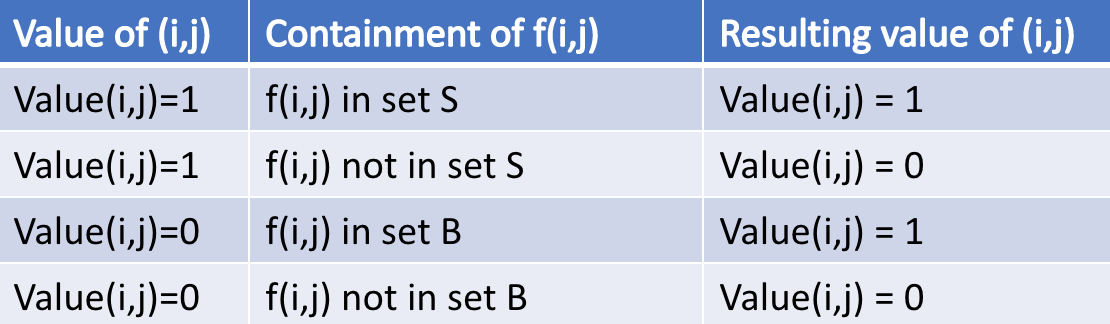
\includegraphics[width=1\linewidth]{EvolutionTable.png}\\

All lattice sites are evolved simultaneously, and a game progresses by continuing to apply these rules to some initial condition.  We can label a game with the terminology of $B \#_1\#_2.../S\#_a\#_b...$, where $B = \{\#_1,\#_2,...\}, S = \{\#_a, \#_b...\}$. In this notation, the Game of Life is $B3/S23$. 

}

\headerbox{Statistical Measures}{name=measures,column=0,below=definitions}{
\textbf{Alive Cell Ratio} Measuring the change in this over the evolution of the system gives a measure of whether a set of rules leads to homogeneity(all alive or all dead), or whether it reaches another equillibrium. \\
\textbf{Displacement from Origin} The mean displacement from the center of the lattice of all alive cells will give a measure of the symmetry of the system. This will be important when we attempt to implement bias. \\
\textbf{Speed} The speed at which a configuration moves away from the origin(defined to be the maximal displacement divided by its evolution time) will be very important when discussing the divergence of configurations and of rule sets more generally.  \\

}

\headerbox{References}{name=references,column=0,below=measures}{
\smaller													% Make the whole text smaller
\vspace{-0.4em} 										% Save some space at the beginning
\bibliographystyle{plain}							% Use plain style
\renewcommand{\section}[2]{\vskip 0.05em}		% Omit "References" title
\begin{thebibliography}{1}							% Simple bibliography with widest label of 1
\itemsep=-0.01em										% Save space between the separation
\setlength{\baselineskip}{0.4em}					% Save space with longer lines
\bibitem{prevWork1} Laszlo Gulyas, Richard Legendi: \emph{Effects of Sample Duration on Network Statistics in Elementary Models of Dynamic Networks}, International Conference on Computational Science, Singapore (2011) 
\bibitem{prevWork2} Laszlo Gulyas, Susan Khor, Richard Legendi and George Kampis \emph{Cumulative Properties of Elementary Dynamic Networks}, The International Sunbelt Social Network Conference XXXI (2011)

\end{thebibliography}
}


\headerbox{Neighbor Weight Biasing}{name=neighbor,span=1,column=1,row=0}{
A key aspect of the Game of Life is that it has equal neighbor weights, such that $w_0 = w_1 =  \dots = w_7 =1$. This means that the evolution of a configuration has no special preference for any direction, meaning that symmetric configurations will remain symmetric. If we allow variation of these weights, we see that we can implement various types of bias on the evolution of our system.\\

We can use a symmetric initial configuration and the rule set $B34S23$ to demonstrate this bias. For equal weights on the left and an increase in weighting of the upper left corner on the right, we have the following evolutions.

 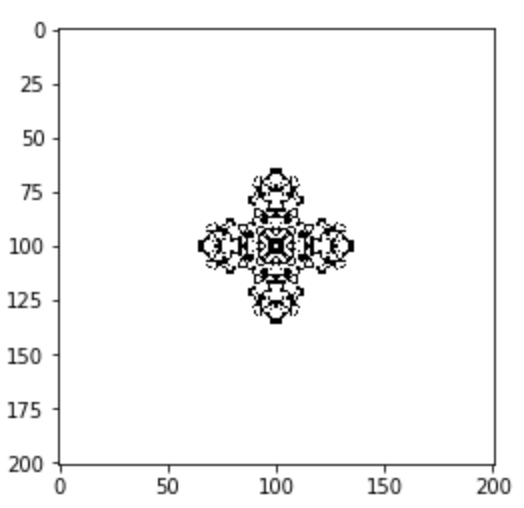
\includegraphics[width=0.4\linewidth]{SymmetricFinal}   vs.
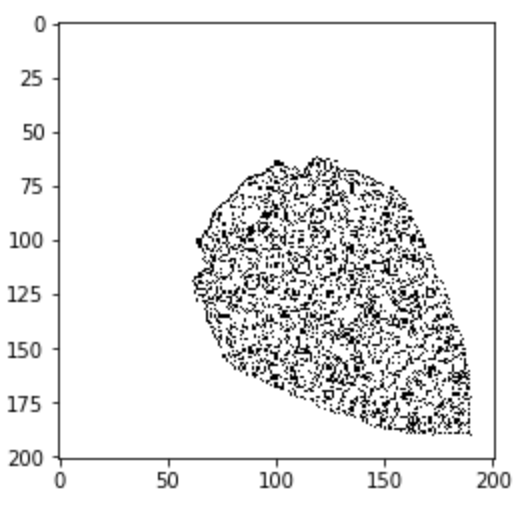
\includegraphics[width=0.4\linewidth]{AsymmetricFinal}

We can clearly see that the symmetric one will have a mean displacement of zero, while the asymmetric one will have a large mean displacement, but what is most interesting is the differing rates at which these two systems evolve, both from a number of alive cells and a speed perspective. If we look




}
\headerbox{Particle in a Box}{name=boundary,span=1,column=2,row=0}{
	Another aspect of the Game of Life is that it is played on a periodic boundary. This allows for moving features, like gliders, and expanding features to increase without bound. One interesting alternative to this is to create a boundary that confines the features to a lattice of fixed size. For this simulation, we shall use 
	We can use a symmetric initial configuration and the rule set $B34S23$ to demonstrate this bias. For equal weights, we have the following evolution.
	
	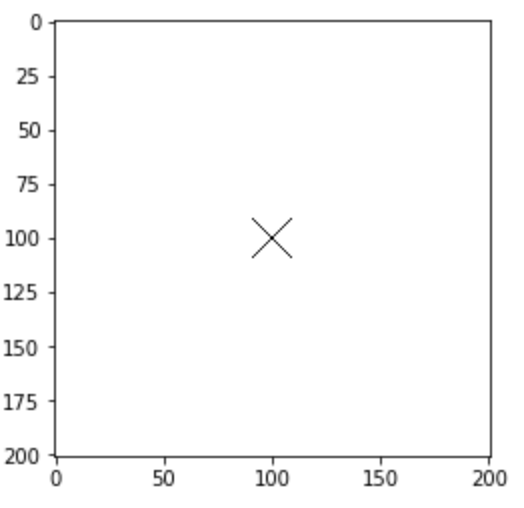
\includegraphics[width=0.4\linewidth]{InitialCondition} $\to$ 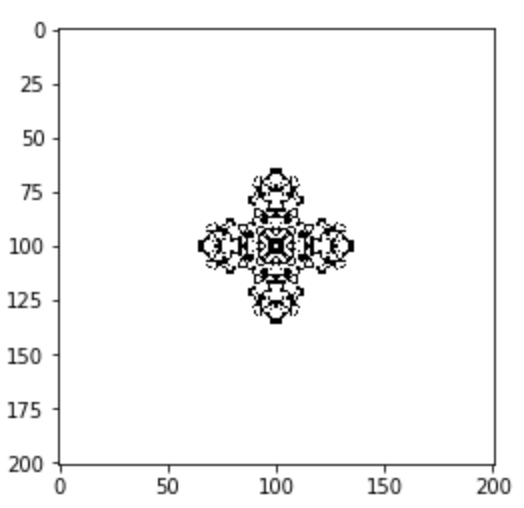
\includegraphics[width=0.4\linewidth]{SymmetricFinal}
	
	We see that this preserves the symmetry of the system. However, if we bias the upper left hand corner, which corresponds to $w_1 = w_3 = 2, w_0 = 3$, then we see very different behavior.
	
	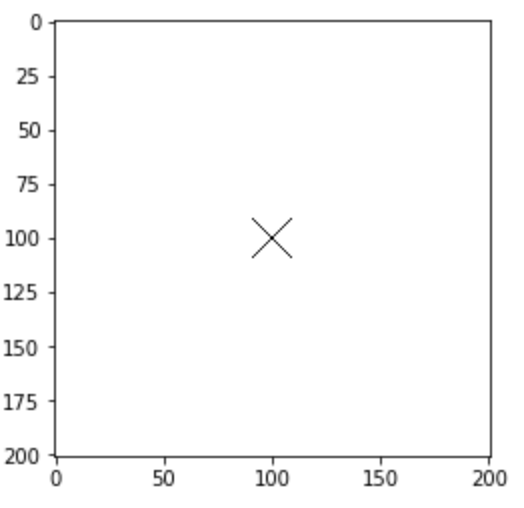
\includegraphics[width=0.4\linewidth]{InitialCondition} $\to$
	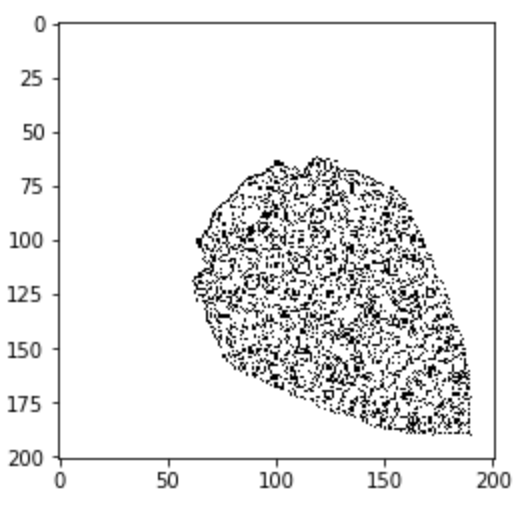
\includegraphics[width=0.4\linewidth]{AsymmetricFinal}
	
	
	
	
	
	
}

\headerbox{Degree Distribution Radically Changes}
{name=degreeDistribution,span=2,column=1,below=neighbor,above=bottom}{
Degree distributions are exceptionally sensitive to the length of the aggregation window. \textbf{The same dynamic network may produce a normal, lognormal or even power law distribution for different aggregation lenghts.} The digree distribution of the snapshot and cumulative network is inherently different. The following surfaces show the CPA model until it approaches the complete network.
\vspace{-0.2em}
\begin{center}
	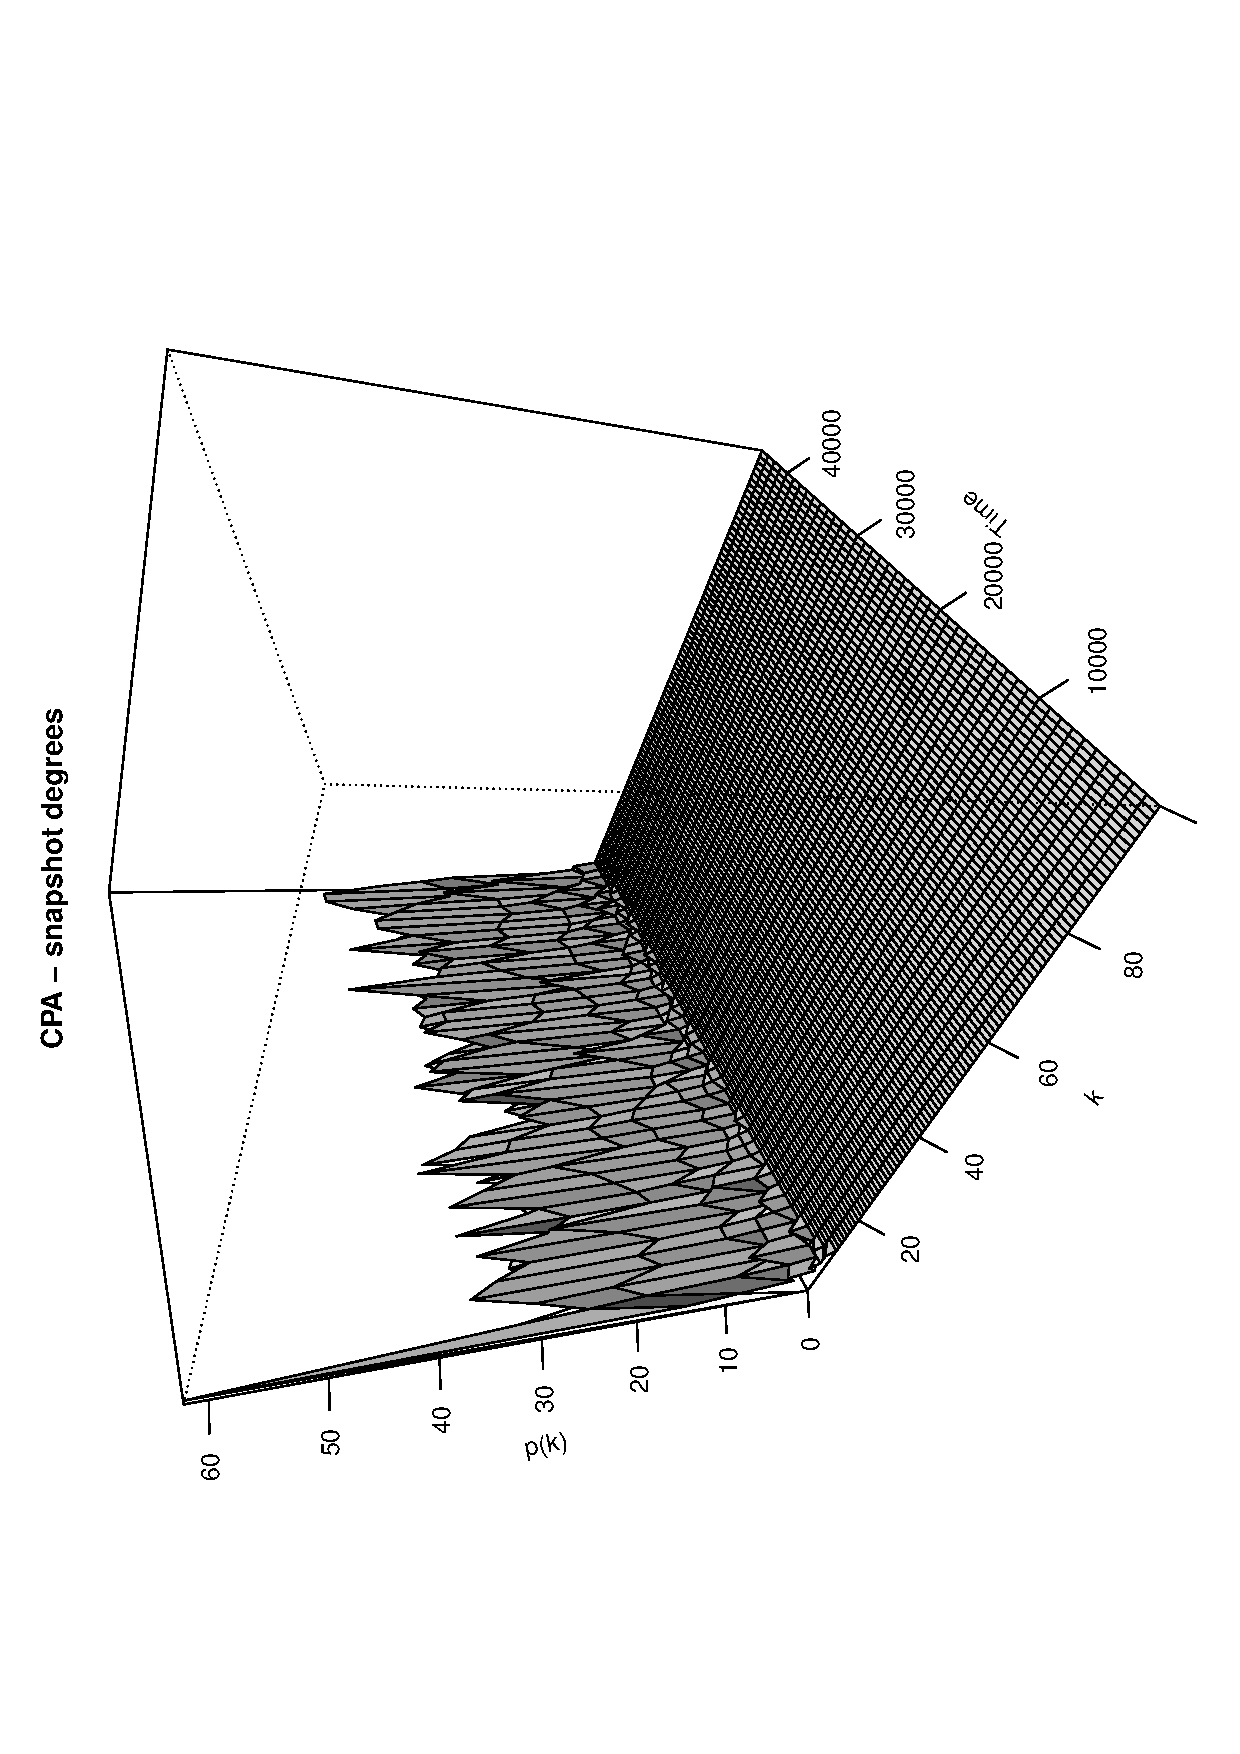
\includegraphics[angle=-90,width=0.49\linewidth]{CPA_3d_snapshot}
	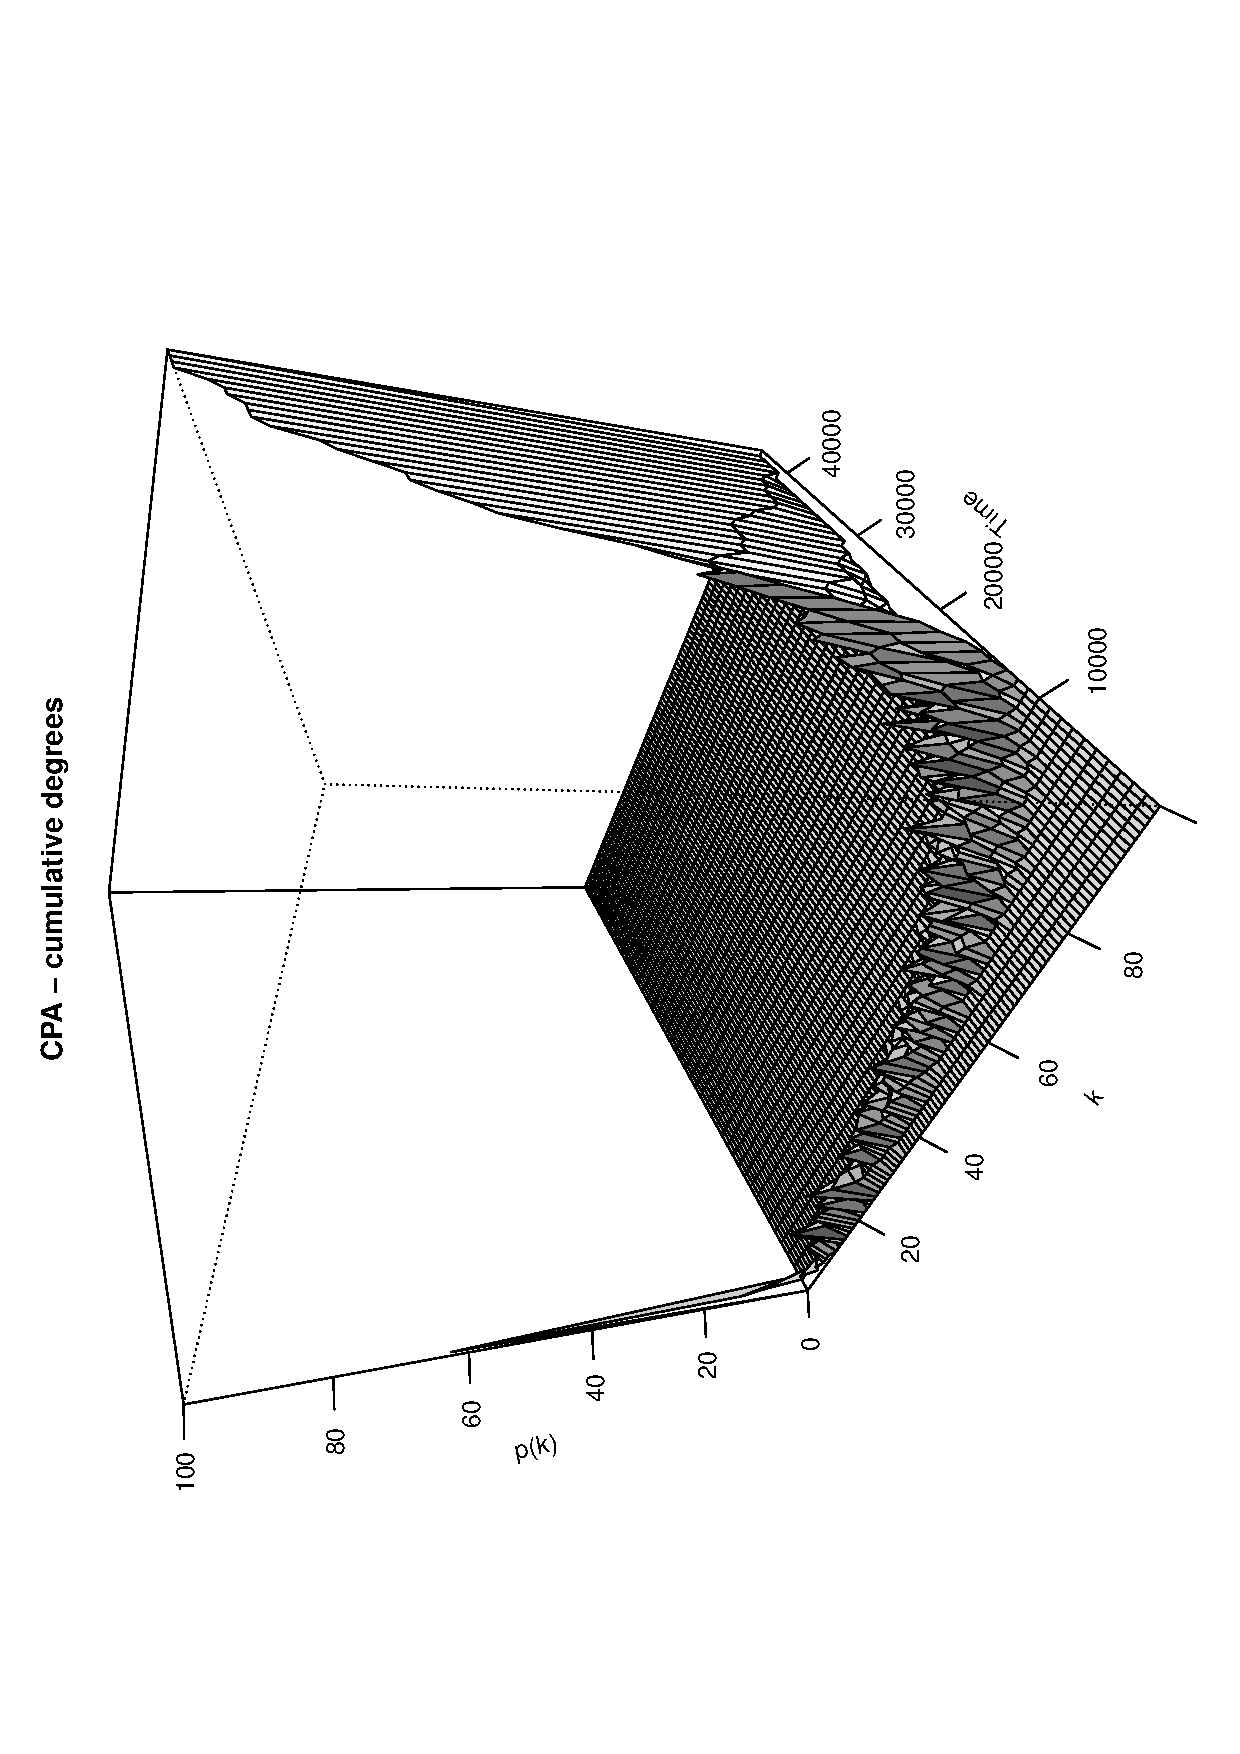
\includegraphics[angle=-90,width=0.49\linewidth]{CPA_3d_cumulative}
\end{center}
\vspace{-0.2em}
Taking slices of the cumulative 3D charts shows us how the degree distribution changes. The log-log charts below show the progression of these changes as the aggregation window gets larger.
\vspace{-0.2em}
\begin{center}
	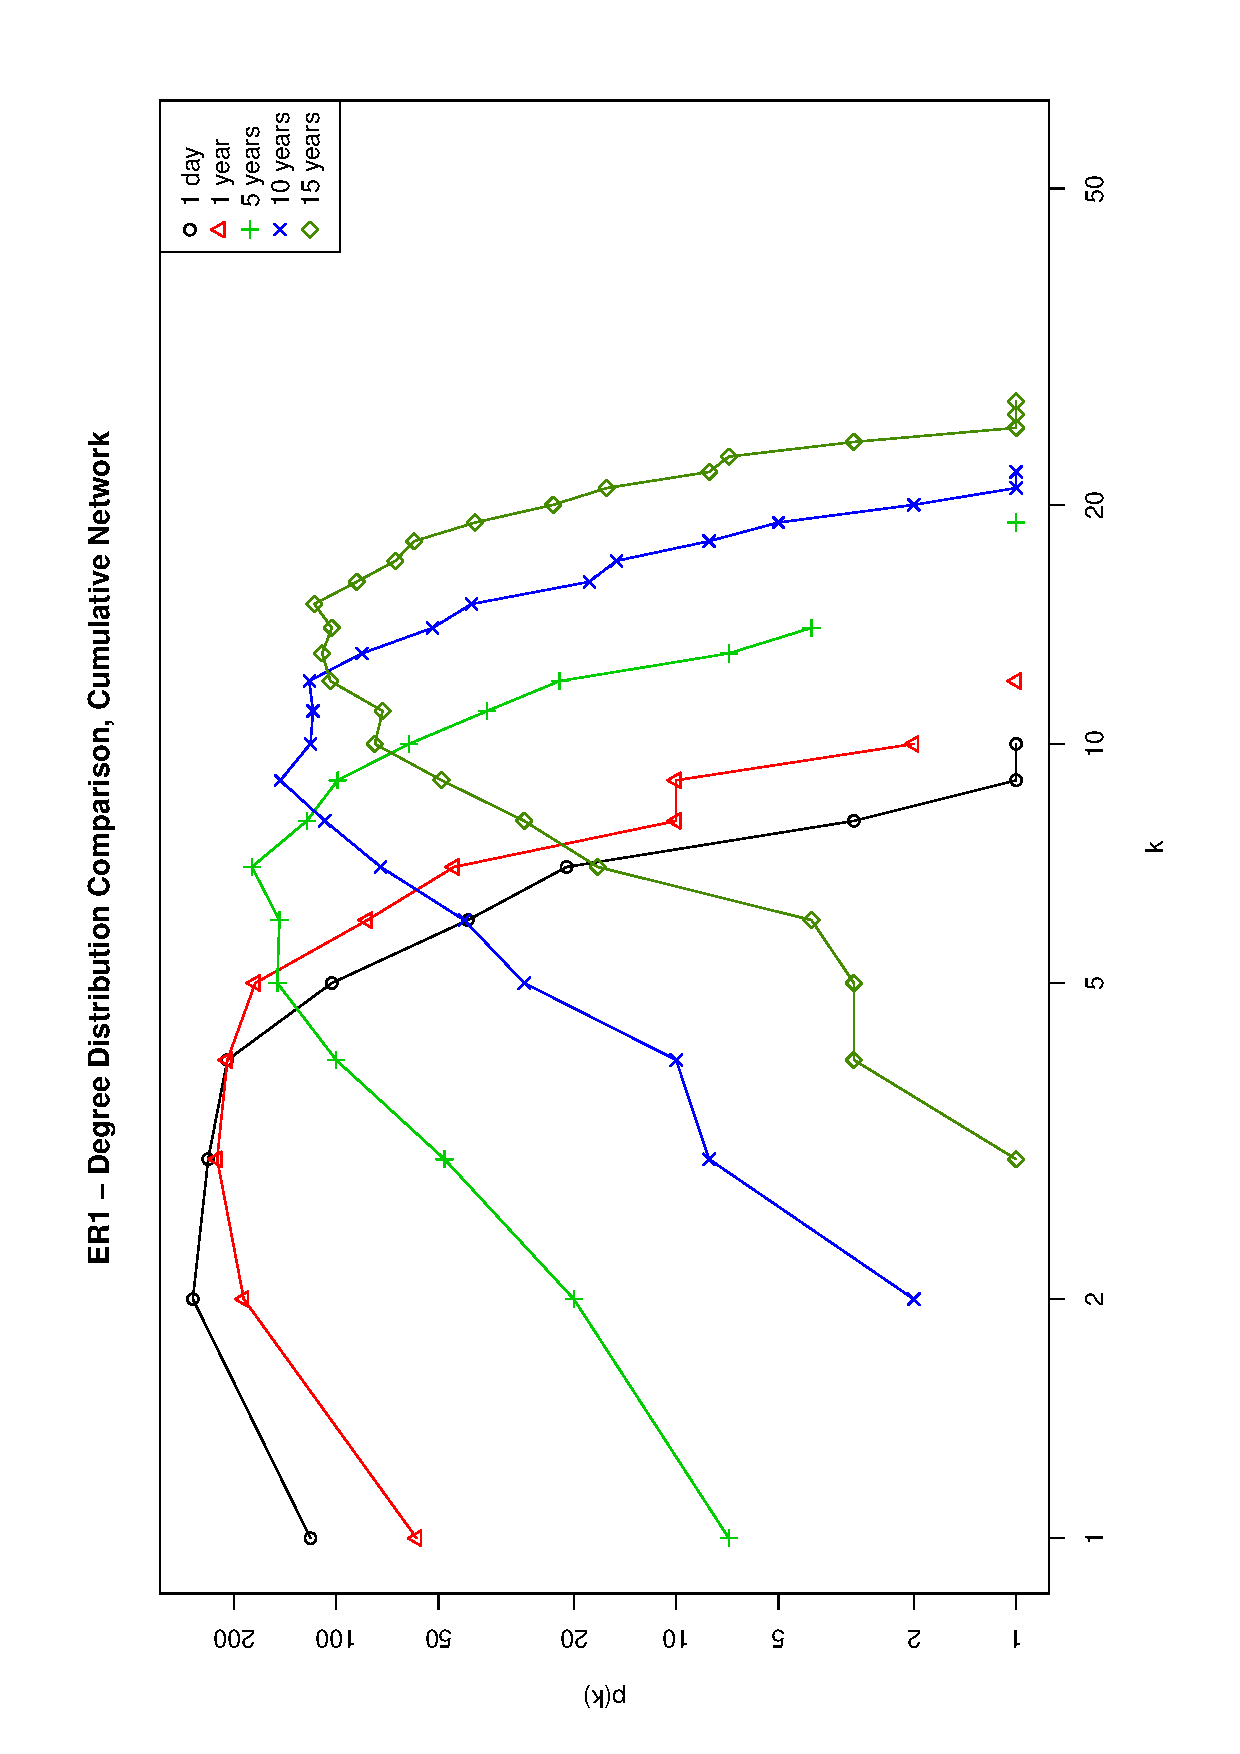
\includegraphics[angle=-90,width=0.49\linewidth]{ER1_cumulativeDegrees}
	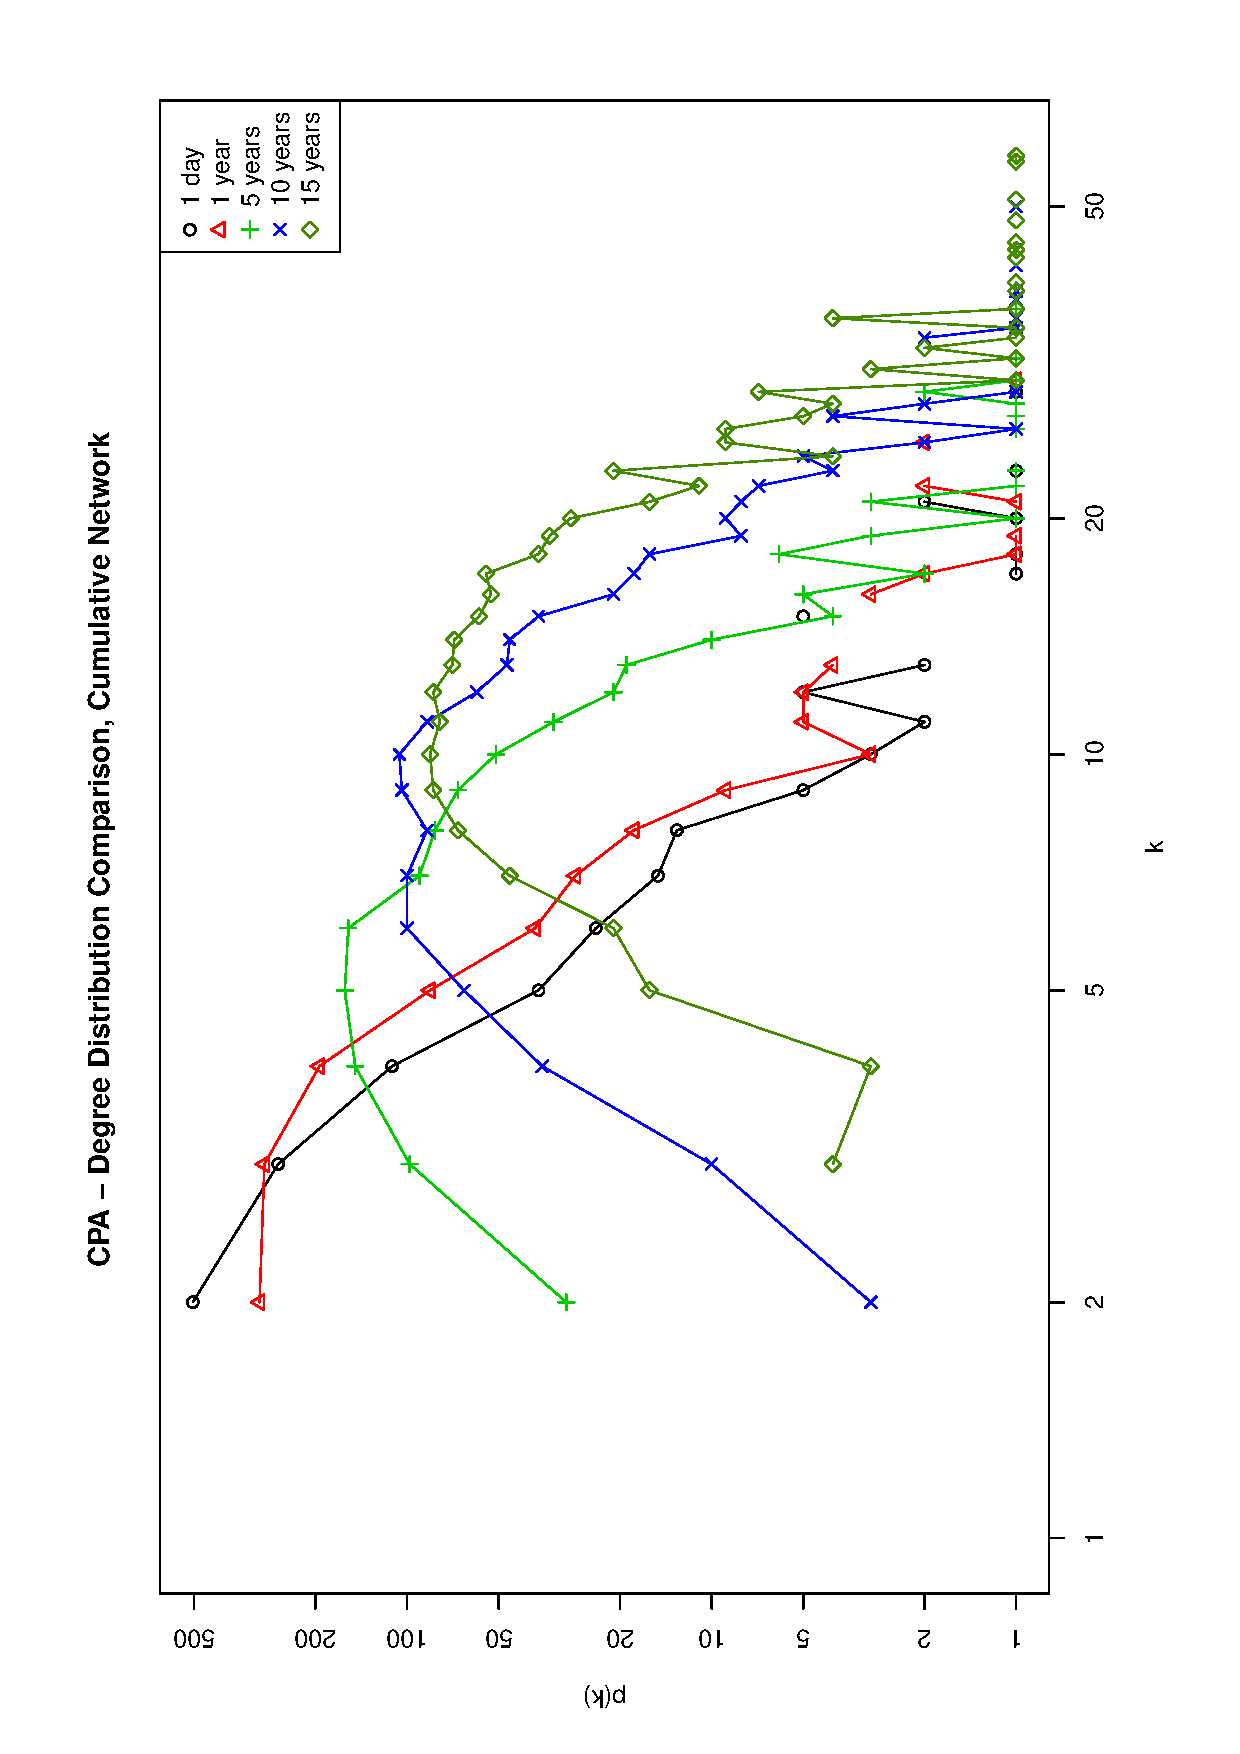
\includegraphics[angle=-90,width=0.49\linewidth]{CPA_cumulativeDegrees}
\end{center}
}

\end{poster}
\end{document}
